% Drawing 74/05-6 -- folder 74, batch 05, archive page 83 (PDF page 84).
% Transcription: Rangée de graphes : un point, un segment, un carré, un hexagone, un pentagone, deux segments (dans un ovale), chacun avec une flèche vers le bas ; sous le dernier, un sablier (bitriangle). À gauche, entouré, un hexagone contenant un carré et une croix.
% Kind: row of graphs with arrows; circled hexagon. Method 2 (schematic redraw from the facsimile). Status: ok.
% Notes: A point, a segment, a square, a hexagon, a pentagon, two segments in an oval, each with an arrow downwards; under the last an hourglass (bitriangle). At the left, circled, a hexagon containing a square and a cross. The handwriting under the row is text.
% Coordinates: 1 unit = 1 mm = 1/100 of the crop width (bbox in page fractions: [0.1, 0.18, 0.66, 0.32]).
% Redrawn by Claude (claude-opus-5-5), issue #73, 2026-11-07; not checked by a human; not compiled (no TeX in the session).
% Rights: reproduces part of the work -- behind RENDER_TRANSCRIPTS, never published by itself.
\documentclass[tikz,border=3pt]{standalone}
\usepackage{amsmath,amssymb}
\usetikzlibrary{patterns,arrows.meta}
\tikzset{pencil/.style={black!45}, struck/.style={black!35}, mark/.style={circle,draw,inner sep=1.3pt}, pt/.style={circle,fill,inner sep=0.9pt}, opt/.style={circle,draw,fill=white,inner sep=1.1pt}}
\begin{document}
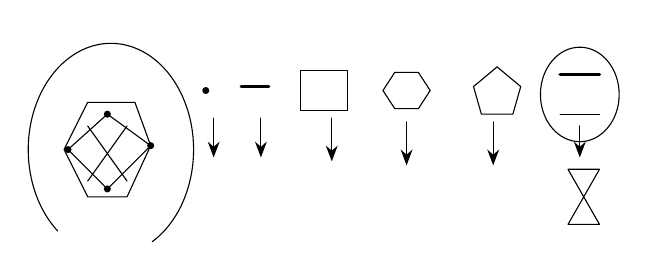
\begin{tikzpicture}[x=1mm,y=1mm,line cap=round,line join=round,font=\scriptsize]
\draw (17,-15) -- (23,-15) -- (25,-20.5) -- (22,-27) -- (17,-27) -- (14,-21) -- cycle;
\draw (19.5,-16.5) -- (25,-20.5) -- (19.5,-26) -- (14.5,-21) -- cycle;
\draw (17,-18) -- (22,-25);
\draw (22,-18) -- (17,-25);
\node[pt] at (14.5,-21) {};
\node[pt] at (25,-20.5) {};
\node[pt] at (19.5,-16.5) {};
\node[pt] at (19.5,-26) {};
\draw (25.2,-32.7) arc[start angle=-60, end angle=230, x radius=10.5, y radius=13.5];
\node[pt] at (32,-13.5) {};
\draw[-{Stealth[length=2mm]}] (33,-17) -- (33,-22);
\draw[very thick] (36.5,-13) -- (40,-13);
\draw[-{Stealth[length=2mm]}] (39,-17) -- (39,-22);
\draw (44,-11) -- (50,-11) -- (50,-16) -- (44,-16) -- cycle;
\draw[-{Stealth[length=2mm]}] (48,-17) -- (48,-22.5);
\draw (60.5,-13.5) -- (59,-15.8) -- (56,-15.8) -- (54.5,-13.5) -- (56,-11.2) -- (59,-11.2) -- cycle;
\draw[-{Stealth[length=2mm]}] (57.5,-17.5) -- (57.5,-23);
\draw (69,-10.5) -- (72,-13) -- (71,-16.5) -- (67,-16.5) -- (66,-13) -- cycle;
\draw[-{Stealth[length=2mm]}] (68.5,-17.5) -- (68.5,-23);
\draw (79.5,-14) ellipse[x radius=5, y radius=6];
\draw[very thick] (77,-11.5) -- (82,-11.5);
\draw (77,-16.5) -- (82,-16.5);
\draw[-{Stealth[length=2mm]}] (79.5,-18) -- (79.5,-22);
\draw (78,-23.5) -- (82,-23.5) -- (78,-30.5) -- (82,-30.5) -- cycle;
\end{tikzpicture}
\end{document}
